% Options for packages loaded elsewhere
\PassOptionsToPackage{unicode}{hyperref}
\PassOptionsToPackage{hyphens}{url}
%
\documentclass[
]{article}
\usepackage{amsmath,amssymb}
\usepackage{iftex}
\ifPDFTeX
  \usepackage[T1]{fontenc}
  \usepackage[utf8]{inputenc}
  \usepackage{textcomp} % provide euro and other symbols
\else % if luatex or xetex
  \usepackage{unicode-math} % this also loads fontspec
  \defaultfontfeatures{Scale=MatchLowercase}
  \defaultfontfeatures[\rmfamily]{Ligatures=TeX,Scale=1}
\fi
\usepackage{lmodern}
\ifPDFTeX\else
  % xetex/luatex font selection
\fi
% Use upquote if available, for straight quotes in verbatim environments
\IfFileExists{upquote.sty}{\usepackage{upquote}}{}
\IfFileExists{microtype.sty}{% use microtype if available
  \usepackage[]{microtype}
  \UseMicrotypeSet[protrusion]{basicmath} % disable protrusion for tt fonts
}{}
\makeatletter
\@ifundefined{KOMAClassName}{% if non-KOMA class
  \IfFileExists{parskip.sty}{%
    \usepackage{parskip}
  }{% else
    \setlength{\parindent}{0pt}
    \setlength{\parskip}{6pt plus 2pt minus 1pt}}
}{% if KOMA class
  \KOMAoptions{parskip=half}}
\makeatother
\usepackage{xcolor}
\usepackage[margin=1in]{geometry}
\usepackage{graphicx}
\makeatletter
\def\maxwidth{\ifdim\Gin@nat@width>\linewidth\linewidth\else\Gin@nat@width\fi}
\def\maxheight{\ifdim\Gin@nat@height>\textheight\textheight\else\Gin@nat@height\fi}
\makeatother
% Scale images if necessary, so that they will not overflow the page
% margins by default, and it is still possible to overwrite the defaults
% using explicit options in \includegraphics[width, height, ...]{}
\setkeys{Gin}{width=\maxwidth,height=\maxheight,keepaspectratio}
% Set default figure placement to htbp
\makeatletter
\def\fps@figure{htbp}
\makeatother
\setlength{\emergencystretch}{3em} % prevent overfull lines
\providecommand{\tightlist}{%
  \setlength{\itemsep}{0pt}\setlength{\parskip}{0pt}}
\setcounter{secnumdepth}{-\maxdimen} % remove section numbering
\usepackage{booktabs}
\usepackage{longtable}
\usepackage{array}
\usepackage{multirow}
\usepackage{wrapfig}
\usepackage{float}
\usepackage{colortbl}
\usepackage{pdflscape}
\usepackage{tabu}
\usepackage{threeparttable}
\usepackage{threeparttablex}
\usepackage[normalem]{ulem}
\usepackage{makecell}
\usepackage{xcolor}
\ifLuaTeX
  \usepackage{selnolig}  % disable illegal ligatures
\fi
\usepackage{bookmark}
\IfFileExists{xurl.sty}{\usepackage{xurl}}{} % add URL line breaks if available
\urlstyle{same}
\hypersetup{
  pdftitle={Methane Forecasting},
  hidelinks,
  pdfcreator={LaTeX via pandoc}}

\title{Methane Forecasting}
\author{}
\date{\vspace{-2.5em}}

\begin{document}
\maketitle

\section{Preparation}\label{preparation}

\subsection{Deseason Data}\label{deseason-data}

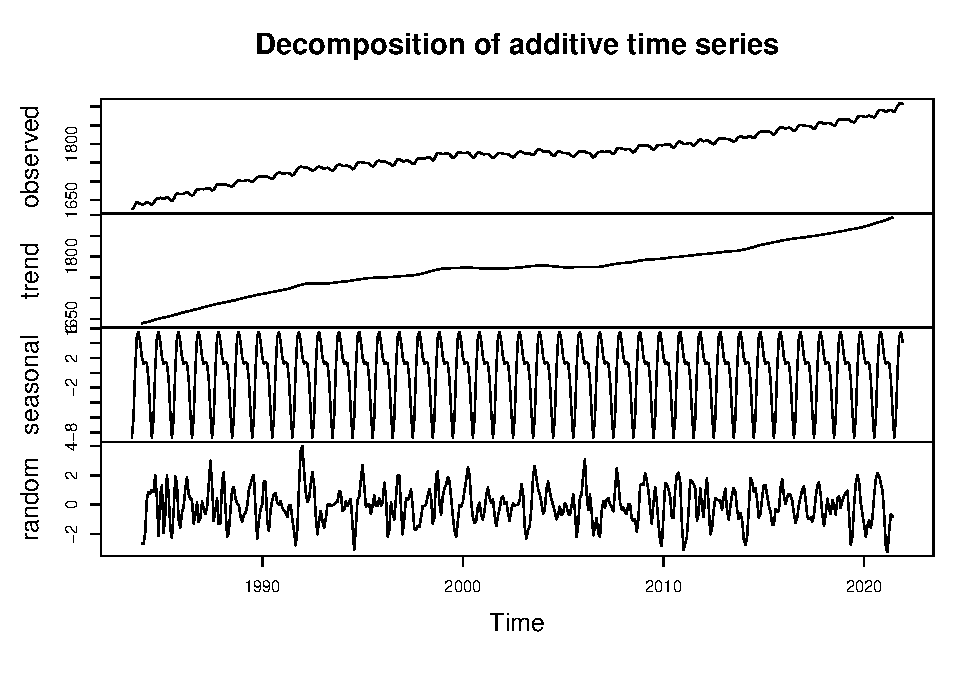
\includegraphics{Methane_Forecasting_files/figure-latex/unnamed-chunk-2-1.pdf}

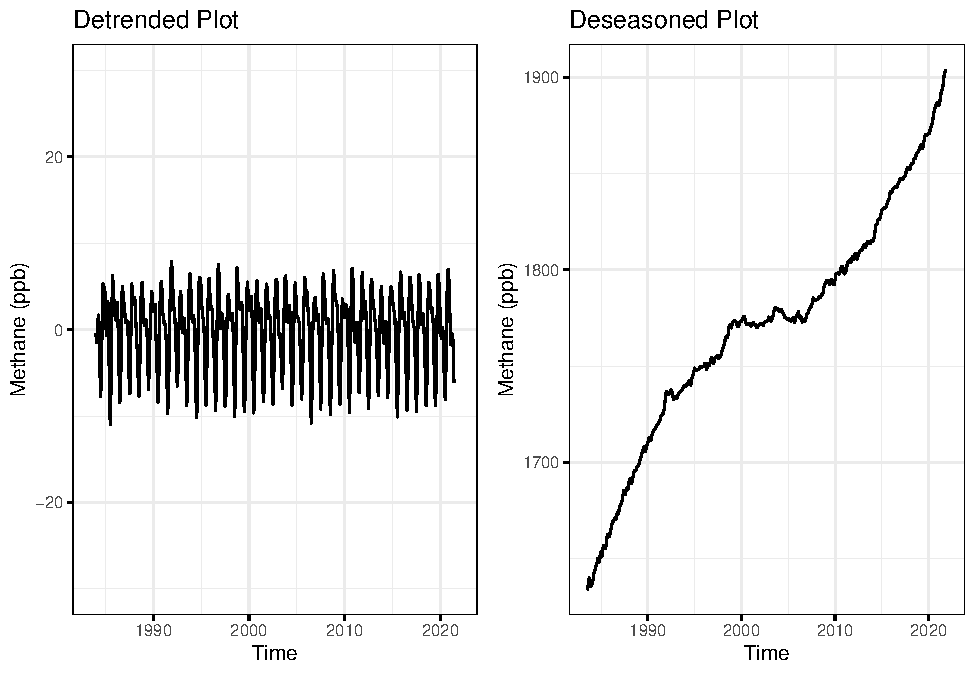
\includegraphics{Methane_Forecasting_files/figure-latex/unnamed-chunk-3-1.pdf}

\subsection{ACF and PACF}\label{acf-and-pacf}

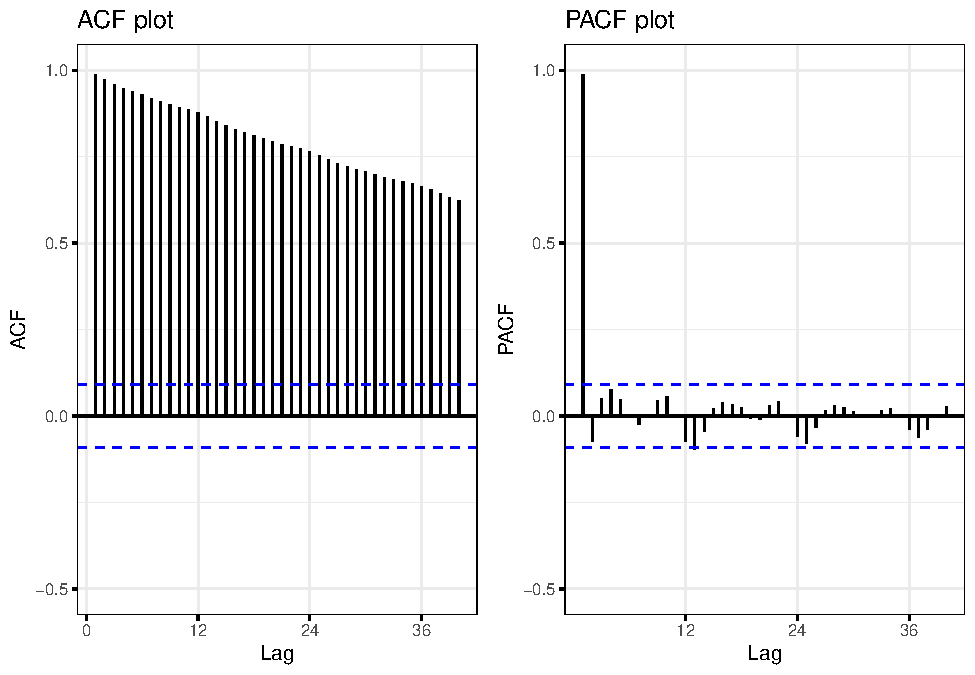
\includegraphics{Methane_Forecasting_files/figure-latex/unnamed-chunk-4-1.pdf}

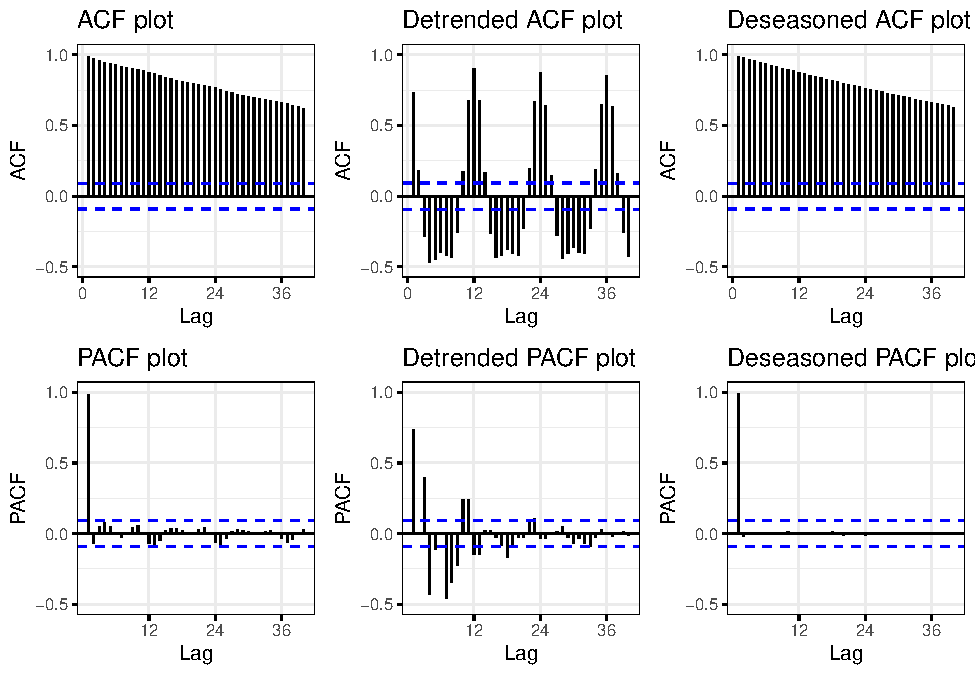
\includegraphics{Methane_Forecasting_files/figure-latex/unnamed-chunk-5-1.pdf}

\subsection{Stationarity Tests}\label{stationarity-tests}

\begin{verbatim}
## [1] "Results from Seasonal Mann-Kendall Test for orginal data"
\end{verbatim}

\begin{verbatim}
## Score =  8432 , Var(Score) = 78964
## denominator =  8664
## tau = 0.973, 2-sided pvalue =< 2.22e-16
\end{verbatim}

\begin{verbatim}
## [1] "Results from Mann-Kendall Test for deseasoned data"
\end{verbatim}

\begin{verbatim}
## Score =  102531 , Var(Score) = 10992237
## denominator =  106491
## tau = 0.963, 2-sided pvalue =< 2.22e-16
\end{verbatim}

\begin{verbatim}
## [1] "Results from ADF test for original data"
\end{verbatim}

\begin{verbatim}
## 
##  Augmented Dickey-Fuller Test
## 
## data:  methane_train_ts
## Dickey-Fuller = -1.5755, Lag order = 7, p-value = 0.7574
## alternative hypothesis: stationary
\end{verbatim}

\begin{verbatim}
## [1] "Results from Spearman Correlation"
\end{verbatim}

\begin{verbatim}
## 
##  Spearman's rank correlation rho
## 
## data:  methane_train_ts and c(1:462)
## S = 169160, p-value < 2.2e-16
## alternative hypothesis: true rho is not equal to 0
## sample estimates:
##       rho 
## 0.9897074
\end{verbatim}

\section{Forecasting Models}\label{forecasting-models}

\subsection{ARIMA}\label{arima}

\begin{verbatim}
## Series: methane_deseasoned 
## ARIMA(5,2,4) 
## 
## Coefficients:
##           ar1      ar2      ar3      ar4      ar5     ma1      ma2      ma3
##       -1.0263  -0.7132  -0.3662  -0.1259  -0.1462  1.3931  -0.4270  -1.3047
## s.e.   0.2188   0.1245   0.1203   0.0717   0.0555  0.2176   0.1859   0.1961
##           ma4
##       -0.4437
## s.e.   0.1835
## 
## sigma^2 = 0.431:  log likelihood = -451.77
## AIC=923.54   AICc=924.03   BIC=964.85
\end{verbatim}

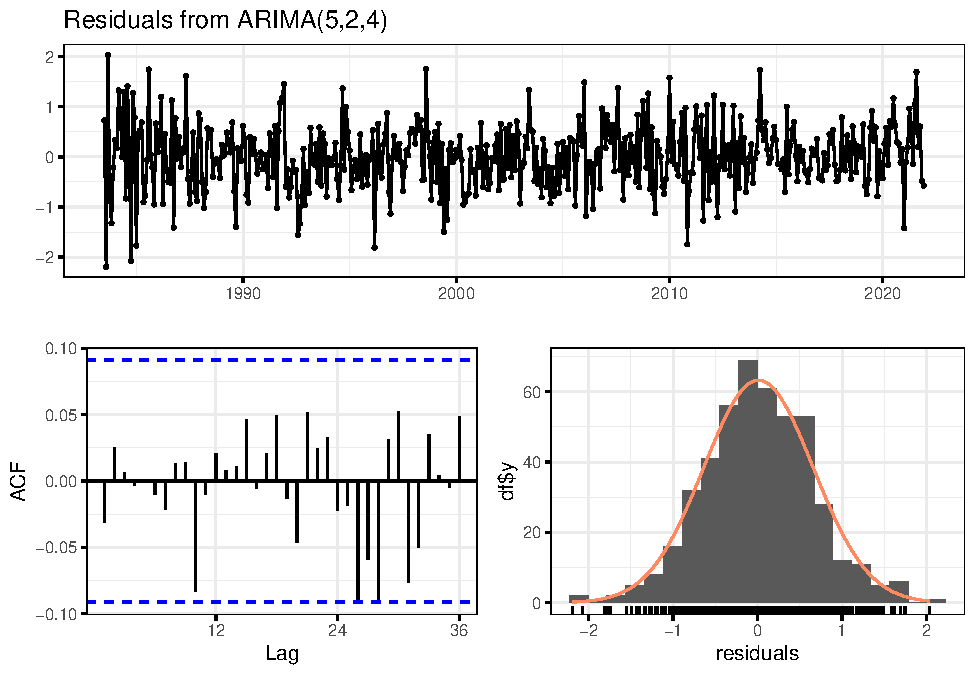
\includegraphics{Methane_Forecasting_files/figure-latex/unnamed-chunk-9-1.pdf}

\begin{verbatim}
## 
##  Ljung-Box test
## 
## data:  Residuals from ARIMA(5,2,4)
## Q* = 10.766, df = 15, p-value = 0.769
## 
## Model df: 9.   Total lags used: 24
\end{verbatim}

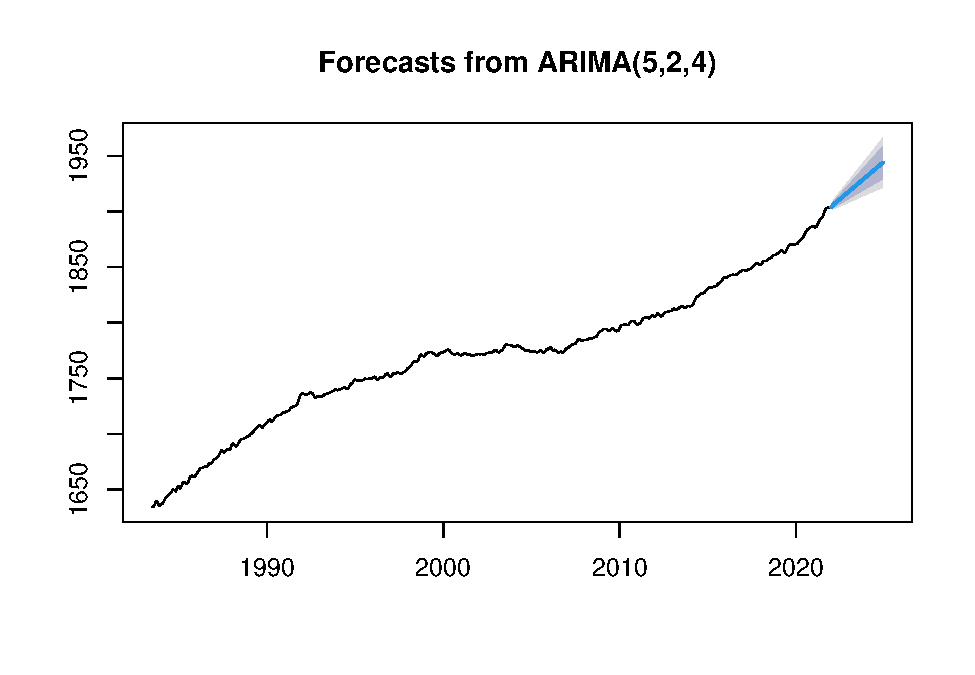
\includegraphics{Methane_Forecasting_files/figure-latex/unnamed-chunk-9-2.pdf}

The ARIMA auto-fit was: ARIMA(5,2,4).

The residuals look pretty good. Otherwise, the residuals are primarily
not significant in the ACF plot and are normally distributed.

\subsection{SARIMA}\label{sarima}

\begin{verbatim}
## Series: methane_train_ts 
## ARIMA(2,1,2)(1,1,1)[12] 
## 
## Coefficients:
##           ar1      ar2     ma1     ma2    sar1     sma1
##       -0.3875  -0.3977  1.7665  0.8226  0.0635  -0.8639
## s.e.   0.0504   0.0470  0.0353  0.0347  0.0740   0.0598
## 
## sigma^2 = 0.5296:  log likelihood = -465.66
## AIC=945.32   AICc=945.57   BIC=974.07
\end{verbatim}

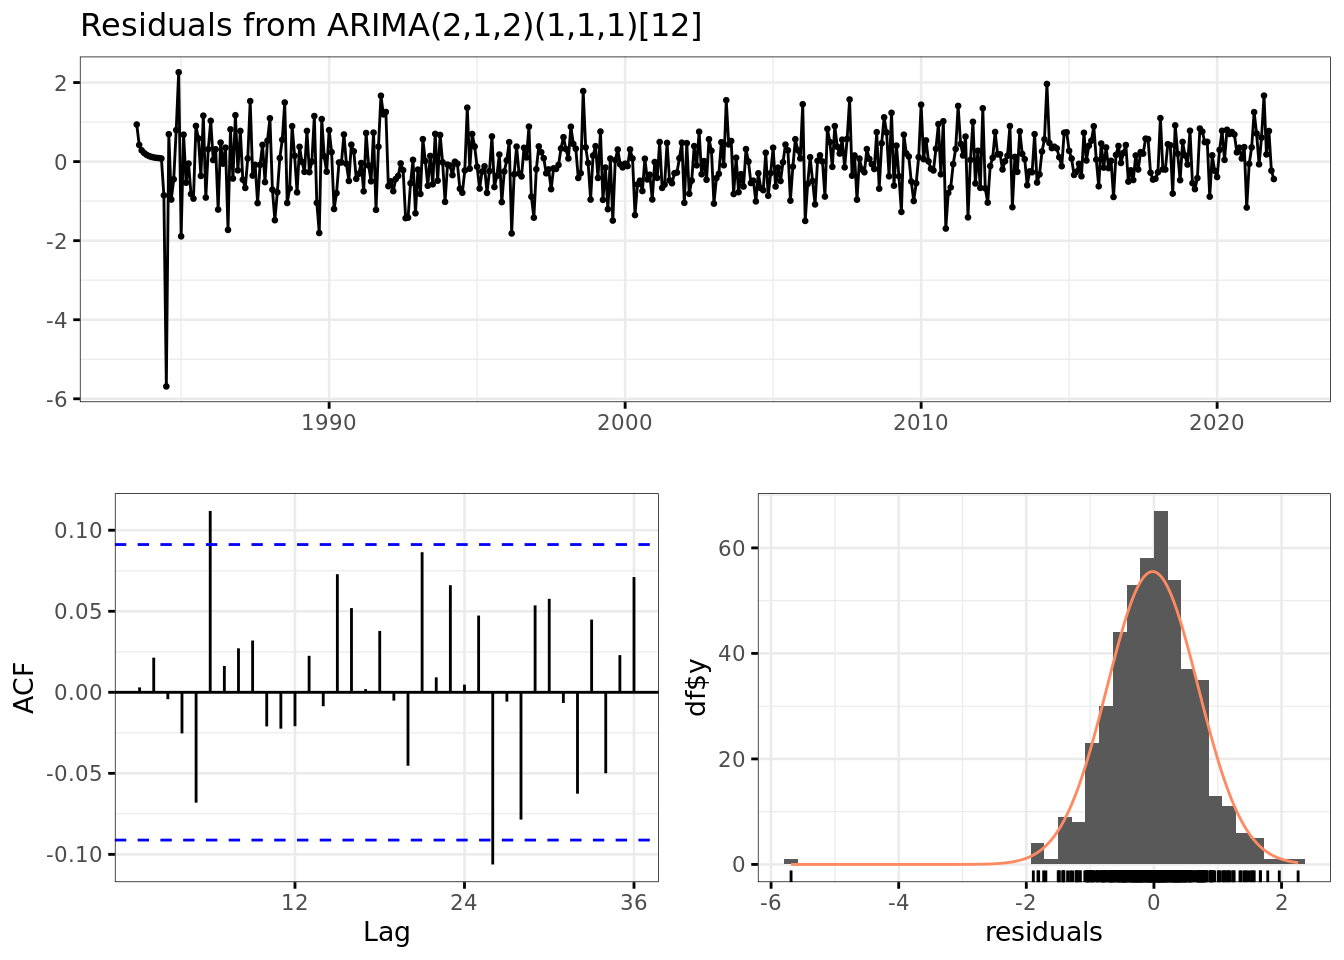
\includegraphics{Methane_Forecasting_files/figure-latex/unnamed-chunk-10-1.pdf}

\begin{verbatim}
## 
##  Ljung-Box test
## 
## data:  Residuals from ARIMA(2,1,2)(1,1,1)[12]
## Q* = 21.848, df = 18, p-value = 0.2388
## 
## Model df: 6.   Total lags used: 24
\end{verbatim}

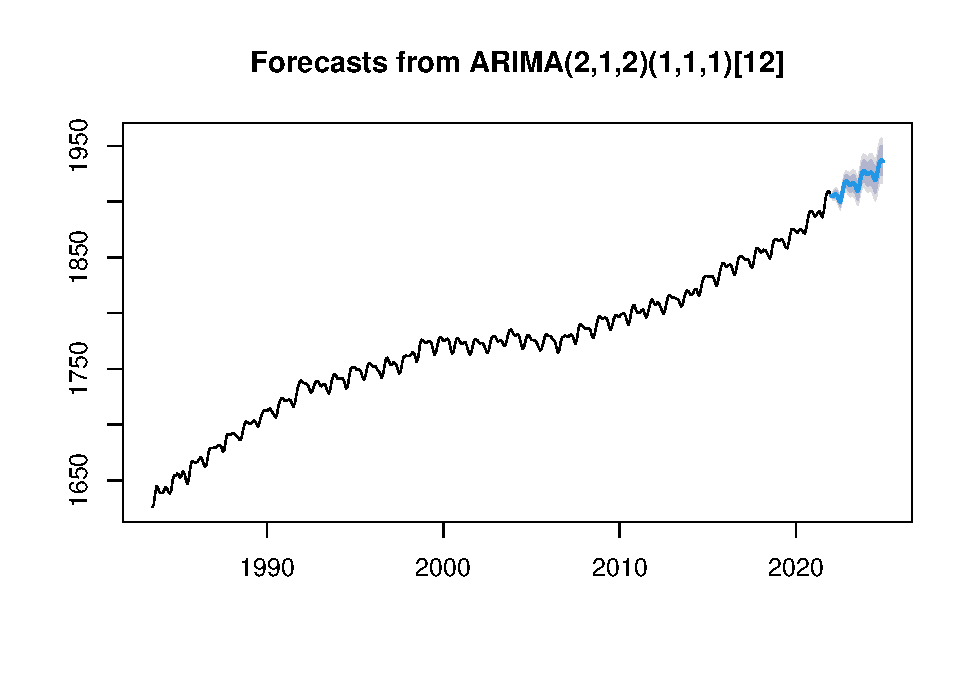
\includegraphics{Methane_Forecasting_files/figure-latex/unnamed-chunk-10-2.pdf}

The SARIMA auto-fit was: ARIMA(2,1,2)(1,1,1){[}12{]}.

The residuals look pretty good. There is one notable outlier. Otherwise,
the residuals are primarily not significant in the ACF plot and are
normally distributed.

\section{Performance Comparison}\label{performance-comparison}

\begin{table}
\centering
\caption{\label{tab:unnamed-chunk-12}Forecast Accuracy}
\centering
\begin{tabular}[t]{l|r|r|r|r|r|r|r}
\hline
  & ME & RMSE & MAE & MPE & MAPE & ACF1 & Theil.s.U\\
\hline
\cellcolor{gray!10}{ARIMA} & \cellcolor{gray!10}{-4.01311} & \cellcolor{gray!10}{8.95048} & \cellcolor{gray!10}{5.72832} & \cellcolor{gray!10}{-0.20938} & \cellcolor{gray!10}{0.29870} & \cellcolor{gray!10}{0.38099} & \cellcolor{gray!10}{1.32701}\\
\hline
\cellcolor[HTML]{d9ead3}{\textbf{SARIMA}} & \cellcolor[HTML]{d9ead3}{\textbf{2.16610}} & \cellcolor[HTML]{d9ead3}{\textbf{5.98814}} & \cellcolor[HTML]{d9ead3}{\textbf{3.83515}} & \cellcolor[HTML]{d9ead3}{\textbf{0.11234}} & \cellcolor[HTML]{d9ead3}{\textbf{0.19989}} & \cellcolor[HTML]{d9ead3}{\textbf{0.02026}} & \cellcolor[HTML]{d9ead3}{\textbf{0.88646}}\\
\hline
\end{tabular}
\end{table}

\end{document}
